\subsubsection{Peridiograma}

\paragraph{Dendrograma de los clústeres obtenidos}

\begin{figure}[H]
    \centering
    
    \subfigure[\textit{HR}]{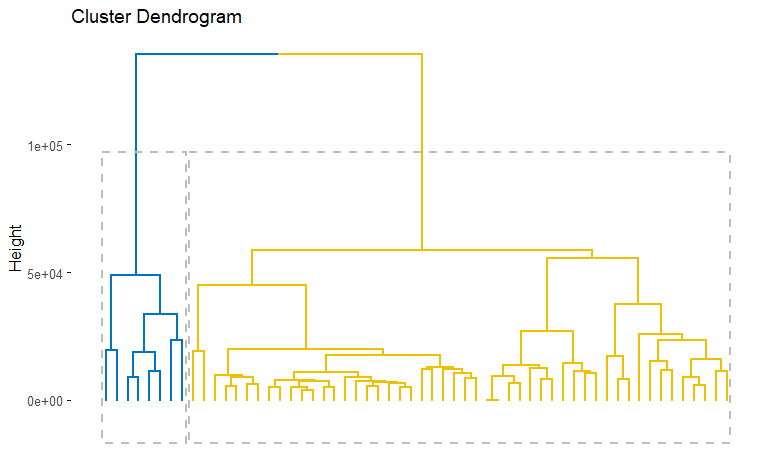
\includegraphics[width=0.45\textwidth]{img/01-1-per.png}}
    \subfigure[\textit{HR\_scaled}]{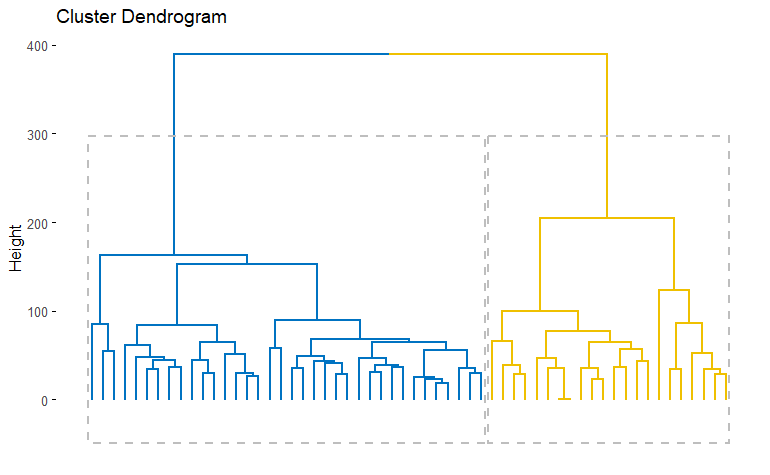
\includegraphics[width=0.45\textwidth]{img/02-1-per.png}}
    \subfigure[\textit{HR\_quantile}]{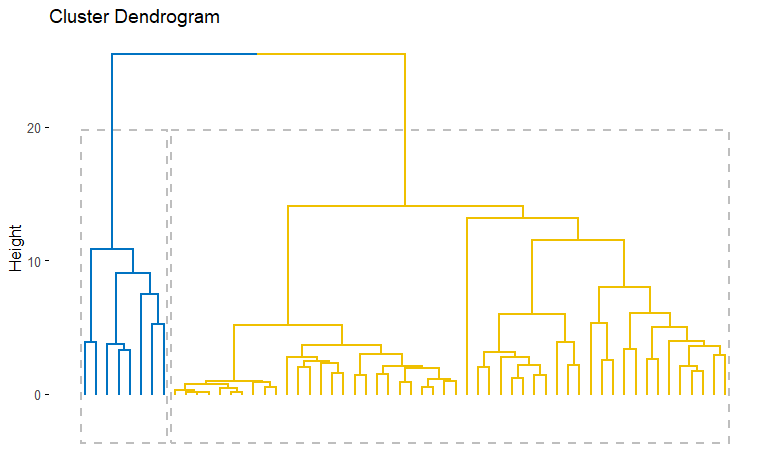
\includegraphics[width=0.5\textwidth]{img/03-1-per.png}}
    \caption{Dendogramas de \textit{HR}, \textit{HR\_scaled} y \textit{HR\_quantile}}
    \label{fig:per_den_fc}
\end{figure}

\begin{figure}[ht]
    \centering
    \subfigure[\textit{SpO2}]{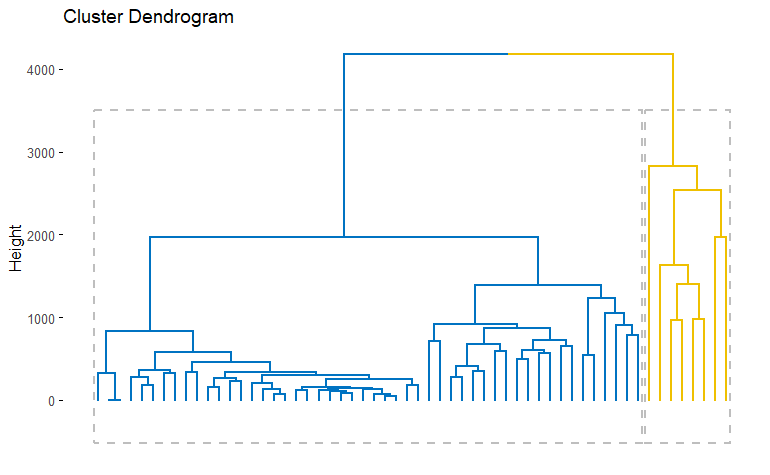
\includegraphics[width=0.5\textwidth]{img/04-1-per.png}}\hfill
    \subfigure[\textit{SpO2\_scaled}]{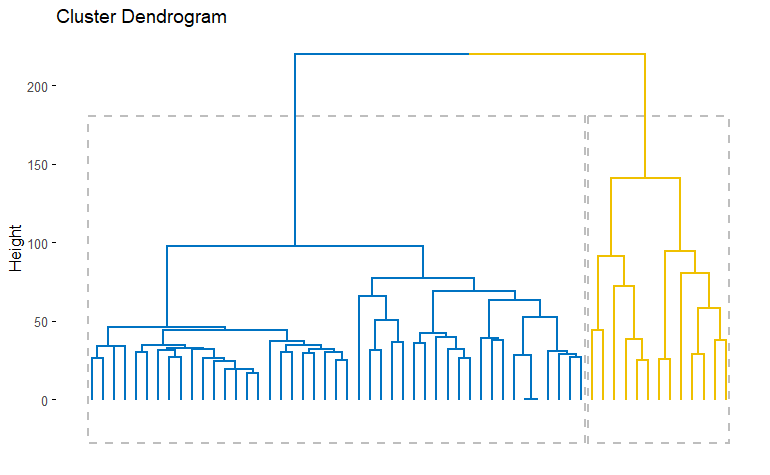
\includegraphics[width=0.5\textwidth]{img/05-1-per.png}}
    \caption{Dendogramas de \textit{SpO2} y \textit{SpO2\_scaled}}\label{fig:per_den_spo2}
\end{figure}

\paragraph{Distribución de los clústeres obtenidos en función de las dos primeras componentes principales}

\begin{figure}[H]
    \centering
    \subfigure[\textit{HR}]{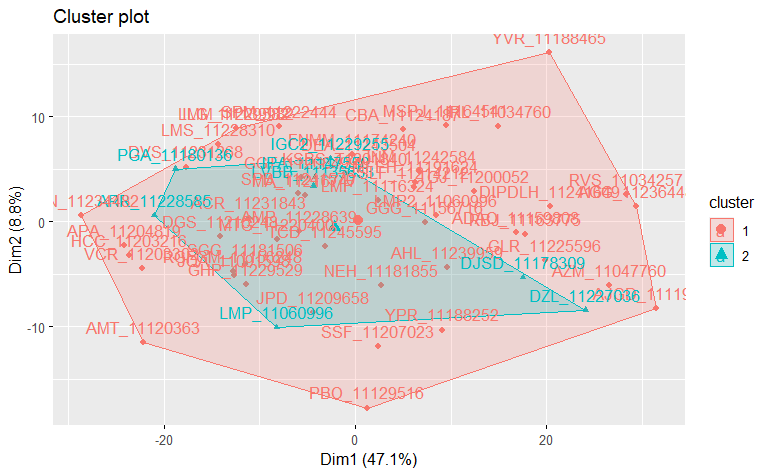
\includegraphics[width=0.45\textwidth]{img/01-2-per.png}}
    \subfigure[\textit{HR\_scaled}]{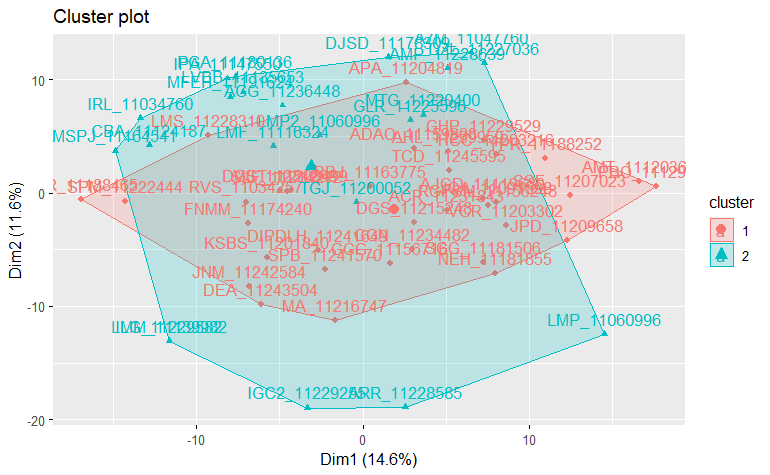
\includegraphics[width=0.45\textwidth]{img/02-2-per.png}}
    \subfigure[\textit{HR\_quantile}]{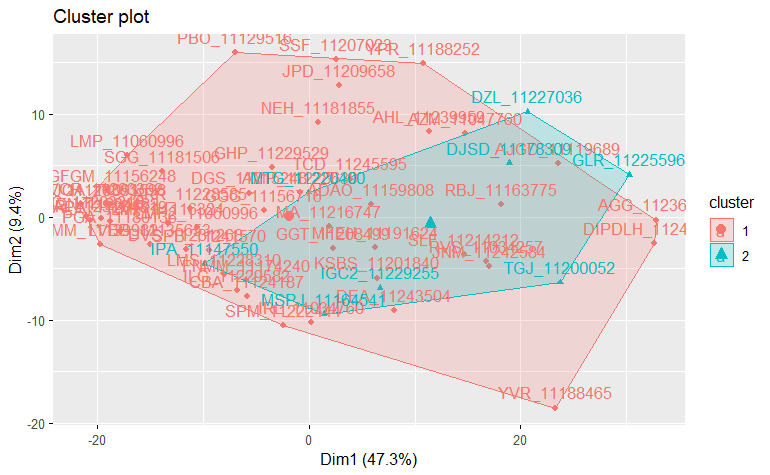
\includegraphics[width=0.5\textwidth]{img/03-2-per.png}}
    \caption{Cluster Plot de \textit{HR}, \textit{HR\_scaled} y \textit{HR\_quantile}}
    \label{fig:per_pc_fc}
\end{figure}

\begin{figure}[ht]
    \centering
    \subfigure[\textit{SpO2}]{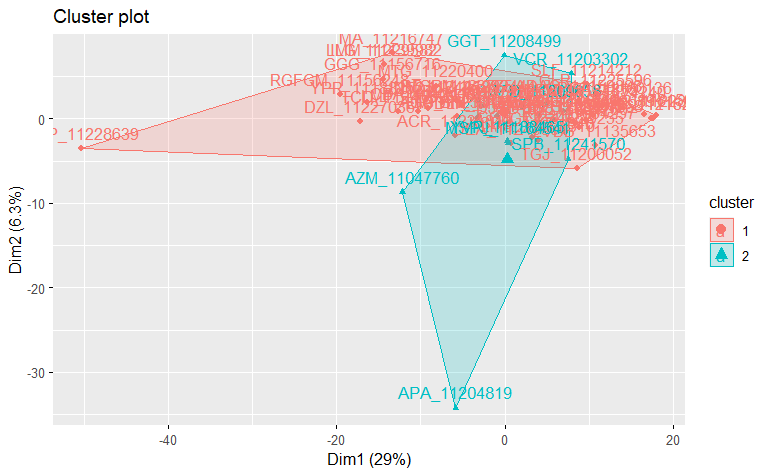
\includegraphics[width=0.5\textwidth]{img/04-2-per.png}}\hfill
    \subfigure[\textit{SpO2\_scaled}]{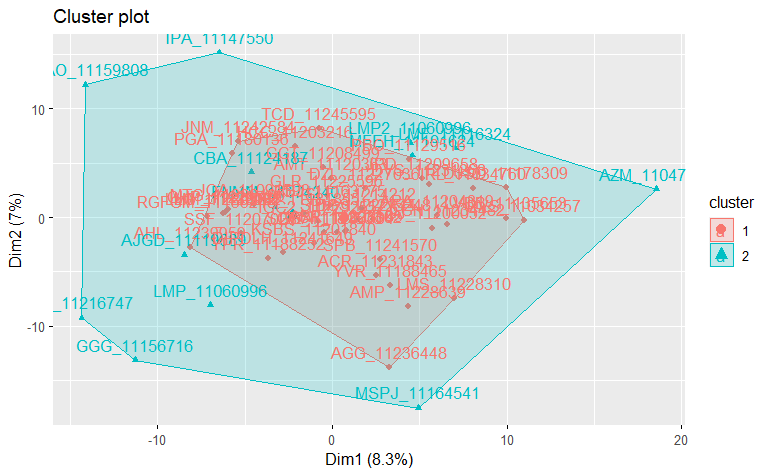
\includegraphics[width=0.5\textwidth]{img/05-2-per.png}}
    \caption{Cluster Plot de \textit{SpO2} y \textit{SpO2\_scaled}}\label{fig:per_pc_spo2}
\end{figure}


\paragraph{Puntuación de Silhouette de los clústeres obtenidos}

\begin{figure}[H]
    \centering
    \subfigure[\textit{HR}]{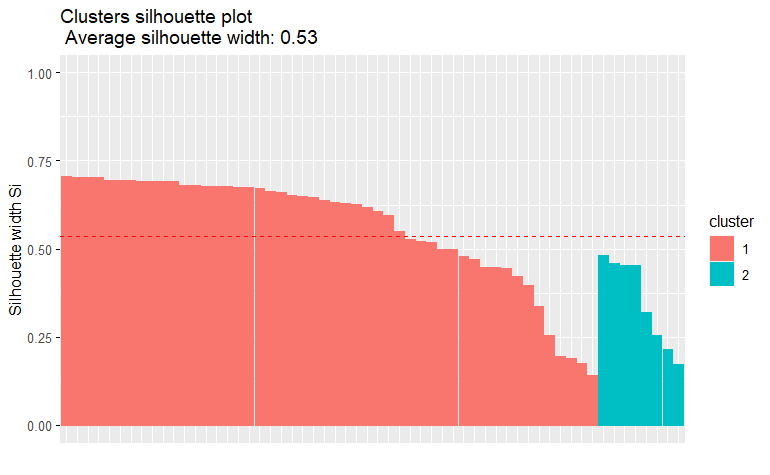
\includegraphics[width=0.45\textwidth]{img/01-3-per.png}}
    \subfigure[\textit{HR\_scaled}]{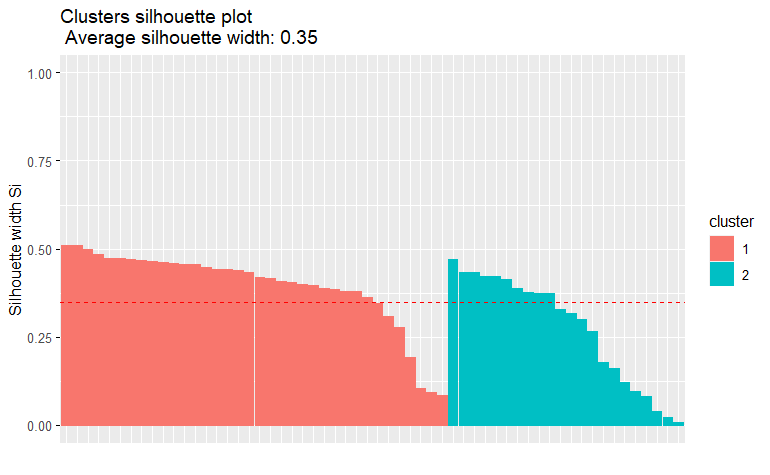
\includegraphics[width=0.45\textwidth]{img/02-3-per.png}}
    \subfigure[\textit{HR\_quantile}]{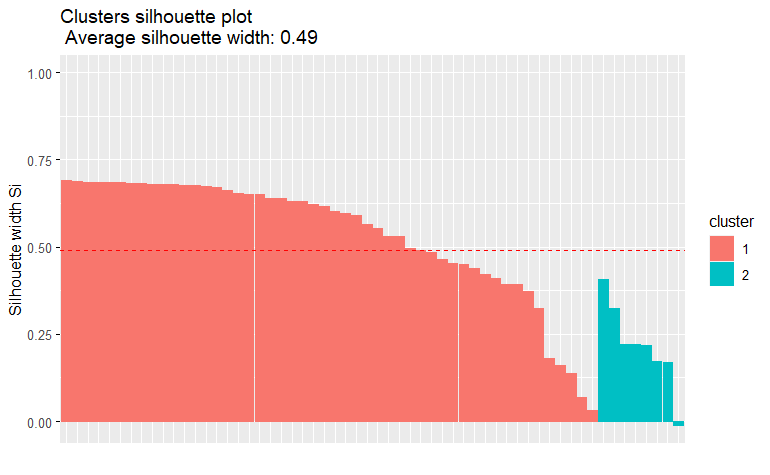
\includegraphics[width=0.5\textwidth]{img/03-3-per.png}}
    \caption{Silhouette Plot de \textit{HR}, \textit{HR\_scaled} y \textit{HR\_quantile}}\label{fig:per_si_fc}
\end{figure}

\begin{figure}[ht]
    \centering
    \subfigure[\textit{SpO2}]{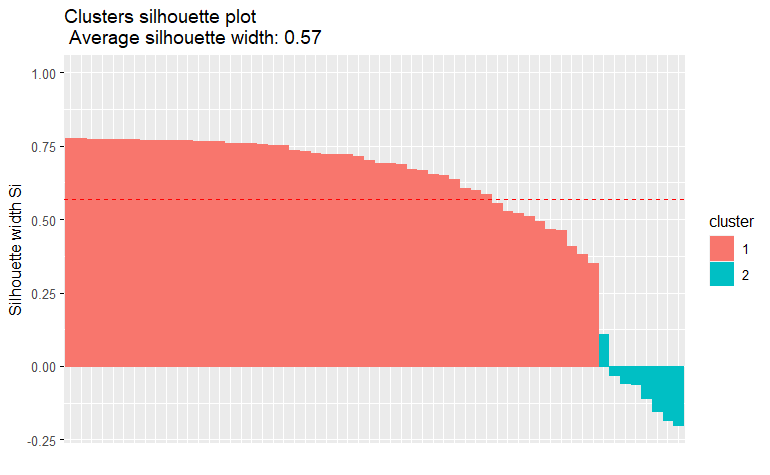
\includegraphics[width=0.5\textwidth]{img/04-3-per.png}}\hfill
    \subfigure[\textit{SpO2\_scaled}]{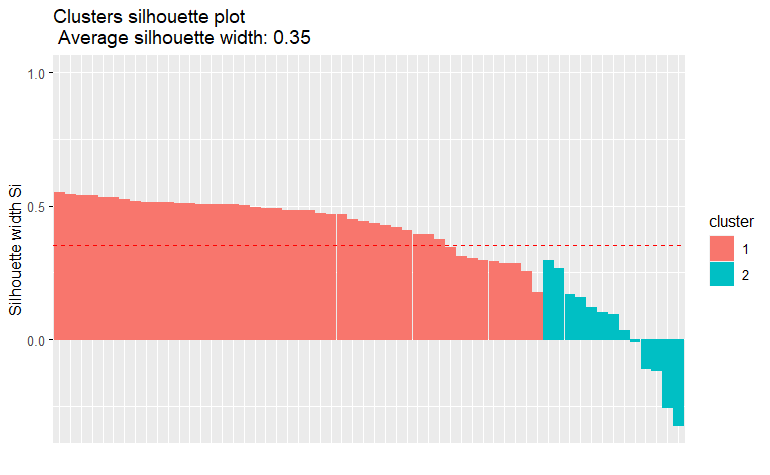
\includegraphics[width=0.5\textwidth]{img/05-3-per.png}}
    \caption{Silhouette Plot de \textit{SpO2} y \textit{SpO2\_scaled}}\label{fig:per_si_spo2}
\end{figure}

\paragraph{Dendograma dividido en dos clústeres según los pacientes que han experimentado OAF}

\begin{figure}[H]
    \centering
    \subfigure[\textit{HR}]{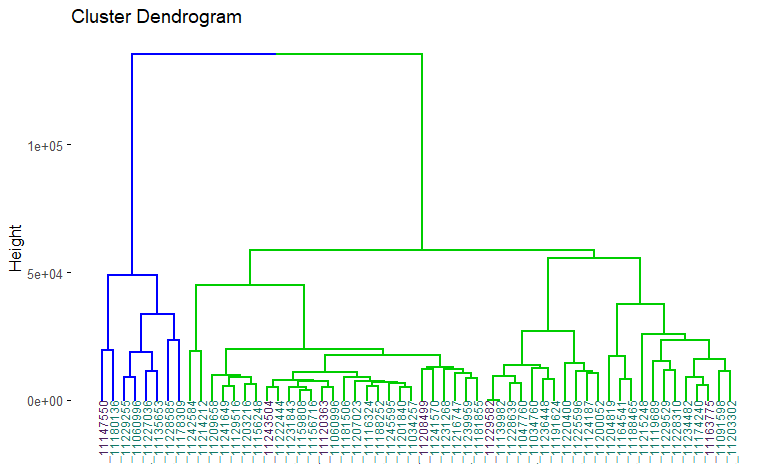
\includegraphics[width=0.45\textwidth]{img/01-4-per.png}}
    \subfigure[\textit{HR\_scaled}]{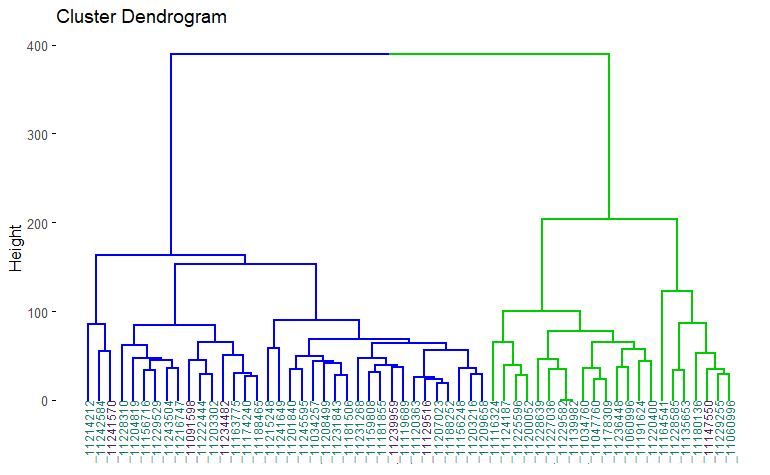
\includegraphics[width=0.45\textwidth]{img/02-4-per.png}}
    \subfigure[\textit{HR\_quantile}]{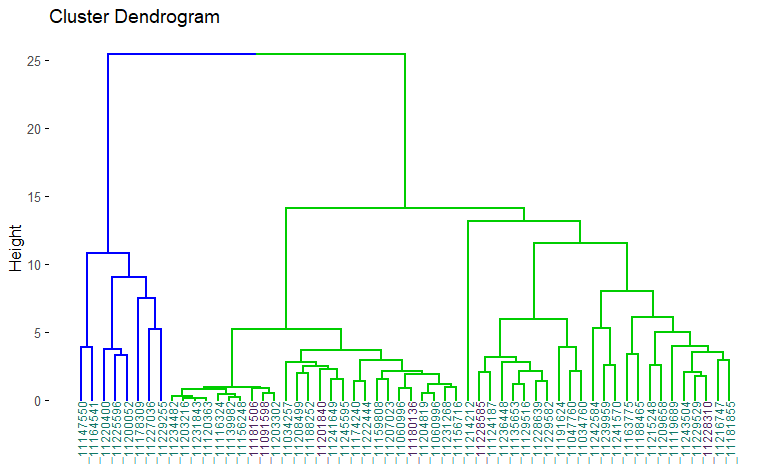
\includegraphics[width=0.5\textwidth]{img/03-4-per.png}}
    \caption{Dendograma Plot k = 2 de \textit{HR}, \textit{HR\_scaled} y \textit{HR\_quantile}}\label{fig:per_ctg_fc}
\end{figure}

\begin{figure}[ht]
    \centering
    \subfigure[\textit{SpO2}]{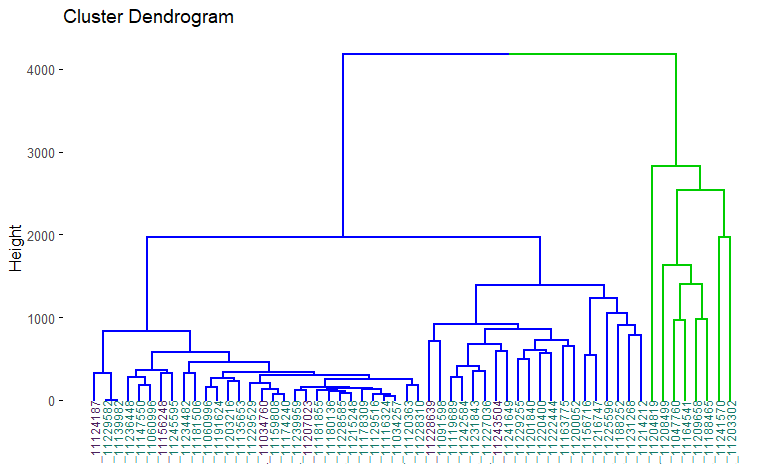
\includegraphics[width=0.5\textwidth]{img/04-4-per.png}}\hfill
    \subfigure[\textit{SpO2\_scaled}]{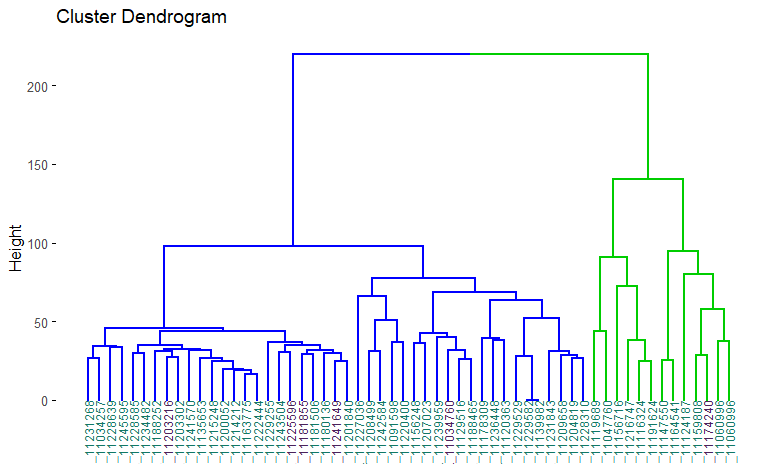
\includegraphics[width=0.5\textwidth]{img/05-4-per.png}}
    \caption{Dendograma Plot k = 2 de \textit{SpO2} y \textit{SpO2\_scaled}}\label{fig:per_ctg_spo2}
\end{figure}

\paragraph{Clasificación mediente Random Forest de los clústeres según las variables \textit{Cuantitativas} y \textit{Cualitativas} de la Tabla~\ref{tabla:variables_estudio_final}}

\begin{figure}[H]
    \centering
    \begin{lstlisting}[frame=single, basicstyle=\small\ttfamily]
        randomForest(formula = CLUSTER ~ ., data = newSMOTE_PER) 
               Type of random forest: classification
                     Number of trees: 500
No. of variables tried at each split: 5

        OOB estimate of  error rate: 6.45%
Confusion matrix:
   1  2 class.error
1 49  1   0.0200000
2  5 38   0.1162791
    \end{lstlisting}
    \caption{Resultado de Random Forest para \textit{HR} utilizando variables \textit{Cuantitativas} y \textit{Cualitativas} de la Tabla~\ref{tabla:variables_estudio_final} y clasificación de clusters k = 2}\label{fig:random_forest_per_result_1}
\end{figure}
\begin{figure}[H]
    \centering
    \begin{lstlisting}[frame=single, basicstyle=\small\ttfamily]
        randomForest(formula = CLUSTER ~ ., data = newSMOTE_PER) 
               Type of random forest: classification
                     Number of trees: 500
No. of variables tried at each split: 5

        OOB estimate of  error rate: 37.93%
Confusion matrix:
   1 2 class.error
1 28 8   0.2222222
2 14 8   0.6363636
    \end{lstlisting}
    \caption{Resultado de Random Forest para \textit{HR\_scaled} utilizando variables \textit{Cuantitativas} y \textit{Cualitativas} de la Tabla~\ref{tabla:variables_estudio_final} y clasificación de clusters k = 2}
    \label{fig:random_forest_per_result_2}
\end{figure}

\begin{figure}[H]
    \centering
    \begin{lstlisting}[frame=single, basicstyle=\small\ttfamily]
        randomForest(formula = CLUSTER ~ ., data = newMWMOTE_PER) 
               Type of random forest: classification
                     Number of trees: 500
No. of variables tried at each split: 5

        OOB estimate of  error rate: 4.3%
Confusion matrix:
   1  2 class.error
1 47  3  0.06000000
2  1 42  0.02325581
    \end{lstlisting}
    \caption{Resultado de Random Forest para \textit{HR\_quantile} utilizando variables \textit{Cuantitativas} y \textit{Cualitativas} de la Tabla~\ref{tabla:variables_estudio_final} y clasificación de clusters k = 2}
    \label{fig:random_forest_per_result_3}
\end{figure}

\begin{figure}[H]
    \centering
    \begin{lstlisting}[frame=single, basicstyle=\small\ttfamily]
        randomForest(formula = CLUSTER ~ ., data = newSMOTE_PER) 
               Type of random forest: classification
                     Number of trees: 500
No. of variables tried at each split: 5

        OOB estimate of  error rate: 7.53%
Confusion matrix:
   1  2 class.error
1 48  2   0.0400000
2  5 38   0.1162791
    \end{lstlisting}
    \caption{Resultado de Random Forest para \textit{SpO2} utilizando variables \textit{Cuantitativas} y \textit{Cualitativas} de la Tabla~\ref{tabla:variables_estudio_final} y clasificación de clusters k = 2}\label{fig:random_forest_per_result_4}
\end{figure}
\begin{figure}[H]
    \centering
    \begin{lstlisting}[frame=single, basicstyle=\small\ttfamily]
        randomForest(formula = CLUSTER ~ ., data = newSMOTE_PER) 
               Type of random forest: classification
                     Number of trees: 500
No. of variables tried at each split: 5

        OOB estimate of  error rate: 14.29%
Confusion matrix:
   1  2 class.error
1 41  4  0.08888889
2  8 31  0.20512821
    \end{lstlisting}
    \caption{Resultado de Random Forest para \textit{SpO2\_scaled} utilizando variables \textit{Cuantitativas} y \textit{Cualitativas} de la Tabla~\ref{tabla:variables_estudio_final} y clasificación de clusters k = 2}
    \label{fig:random_forest_per_result_5}
\end{figure}

\paragraph{Mean Decrease Accuracy de las 5 primeras variables descriptivas utilizadas en Random Forest}

\begin{table}[H]
    \centering
    \begin{tabular}{lr}
        \toprule
        \textbf{Variable} & \textbf{Mean Decrease Accuracy} \\
        \midrule
        SCORE\_CRUCES\_INGRESO & 8.9852612 \\
        SCORE\_WOOD\_DOWNES\_INGRESO & 5.2582849 \\
        RADIOGRAFIA & 5.1448815 \\
        SAPI\_0\_8h & 4.2663169 \\
        PESO & 2.6165359 \\
        \bottomrule
    \end{tabular}
    \caption{Mean Decrease Accuracy \textit{HR}}
\end{table}

\begin{table}[H]
    \centering
    \begin{tabular}{lr}
        \toprule
        \textbf{Variable} & \textbf{Mean Decrease Accuracy} \\
        \midrule
        PESO & 2.8009743 \\
        RADIOGRAFIA & 2.6058470 \\
        EDAD & 2.4925543 \\
        FR\_0\_8h & 2.4681832 \\
        SCORE\_WOOD\_DOWNES\_INGRESO & 2.0989243 \\
        \bottomrule
    \end{tabular}
    \caption{Mean Decrease Accuracy \textit{HR\_scaled}}
\end{table}

\begin{table}[H]
    \centering
    \begin{tabular}{lr}
        \toprule
        \textbf{Variable} & \textbf{Mean Decrease Accuracy} \\
        \midrule
        SCORE\_WOOD\_DOWNES\_INGRESO & 7.4074045 \\
        SCORE\_CRUCES\_INGRESO & 6.5504895 \\
        SAPI\_0\_8h & 4.0000376 \\
        DIAS\_O2\_TOTAL & 2.9619896 \\
        EDAD & 2.9220530 \\
        \bottomrule
    \end{tabular}
    \caption{Mean Decrease Accuracy \textit{HR\_quantile}} 
\end{table}

\begin{table}[H]
    \centering
    \begin{tabular}{lr}
        \toprule
        \textbf{Variable} & \textbf{Mean Decrease Accuracy} \\
        \midrule
        SCORE\_WOOD\_DOWNES\_INGRESO & 9.4039903 \\
        SCORE\_CRUCES\_INGRESO & 5.8936796 \\
        SAPI\_0\_8h & 2.9363664 \\
        ETIOLOGIA & 2.5904366 \\
        TABACO & 2.4803961 \\
        \bottomrule
    \end{tabular}
    \caption{Mean Decrease Accuracy \textit{SpO2}}
\end{table}

\begin{table}[H]
    \centering
    \begin{tabular}{lr}
        \toprule
        \textbf{Variable} & \textbf{Mean Decrease Accuracy} \\
        \midrule
        SAPI\_0\_8h & 5.9478329 \\
        EDAD & 4.8844865 \\
        PESO & 4.4966094 \\
        SCORE\_WOOD\_DOWNES\_INGRESO & 3.8820332 \\
        SCORE\_CRUCES\_INGRESO & 3.3041235 \\
        \bottomrule
    \end{tabular}
    \caption{Mean Decrease Accuracy \textit{SpO2\_scaled}}
\end{table}


\paragraph{Clasificación mediente Random Forest de los clústeres según Peridiograma utilizada para genear los mismos} 

\begin{figure}[H]
    \centering
    \begin{lstlisting}[frame=single, basicstyle=\small\ttfamily]
        randomForest(formula = CLUSTER ~ ., data = data_frame_merge_PER) 
               Type of random forest: classification
                     Number of trees: 500
No. of variables tried at each split: 21

        OOB estimate of  error rate: 13.79%
Confusion matrix:
   1 2 class.error
1 50 0           0
2  8 0           1
    \end{lstlisting}
    \caption{Resultado de Random Forest para \textit{HR} utilizando Peridiograma y clasificación de clusters k = 2}\label{fig:random_forest_per_result_RF_1}
\end{figure}
\begin{figure}[H]
    \centering
    \begin{lstlisting}[frame=single, basicstyle=\small\ttfamily]
        randomForest(formula = CLUSTER ~ ., data = data_frame_merge_PER) 
               Type of random forest: classification
                     Number of trees: 500
No. of variables tried at each split: 21

        OOB estimate of  error rate: 13.79%
Confusion matrix:
   1  2 class.error
1 35  1  0.02777778
2  7 15  0.31818182
    \end{lstlisting}
    \caption{Resultado de Random Forest para \textit{HR\_scaled} utilizando Peridiograma y clasificación de clusters k = 2}
    \label{fig:random_forest_per_result_RF_2}
\end{figure}

\begin{figure}[H]
    \centering
    \begin{lstlisting}[frame=single, basicstyle=\small\ttfamily]
        randomForest(formula = CLUSTER ~ ., data = data_frame_merge_PER) 
               Type of random forest: classification
                     Number of trees: 500
No. of variables tried at each split: 21

        OOB estimate of  error rate: 13.79%
Confusion matrix:
   1 2 class.error
1 50 0           0
2  8 0           1
    \end{lstlisting}
    \caption{Resultado de Random Forest para \textit{HR\_quantile} utilizando Peridiograma y clasificación de clusters k = 2}
    \label{fig:random_forest_per_result_RF_3}
\end{figure}

\begin{figure}[H]
    \centering
    \begin{lstlisting}[frame=single, basicstyle=\small\ttfamily]
        randomForest(formula = CLUSTER ~ ., data = data_frame_merge_PER) 
               Type of random forest: classification
                     Number of trees: 500
No. of variables tried at each split: 21

        OOB estimate of  error rate: 8.62%
Confusion matrix:
   1 2 class.error
1 50 0       0.000
2  5 3       0.625
    \end{lstlisting}
    \caption{Resultado de Random Forest para \textit{SpO2} utilizando Peridiograma y clasificación de clusters k = 2}\label{fig:random_forest_per_result_RF_4}
\end{figure}
\begin{figure}[H]
    \centering
    \begin{lstlisting}[frame=single, basicstyle=\small\ttfamily]
        randomForest(formula = CLUSTER ~ ., data = data_frame_merge_PER) 
               Type of random forest: classification
                     Number of trees: 500
No. of variables tried at each split: 21

        OOB estimate of  error rate: 12.07%
Confusion matrix:
   1 2 class.error
1 45 0   0.0000000
2  7 6   0.5384615
    \end{lstlisting}
    \caption{Resultado de Random Forest para \textit{SpO2\_scaled} utilizando Peridiograma y clasificación de clusters k = 2}
    \label{fig:random_forest_per_result_RF_5}
\end{figure}

\paragraph{Distribución de la Importancia de Peridiograma}

\begin{figure}[H]
    \centering
    \subfigure[\textit{HR}]{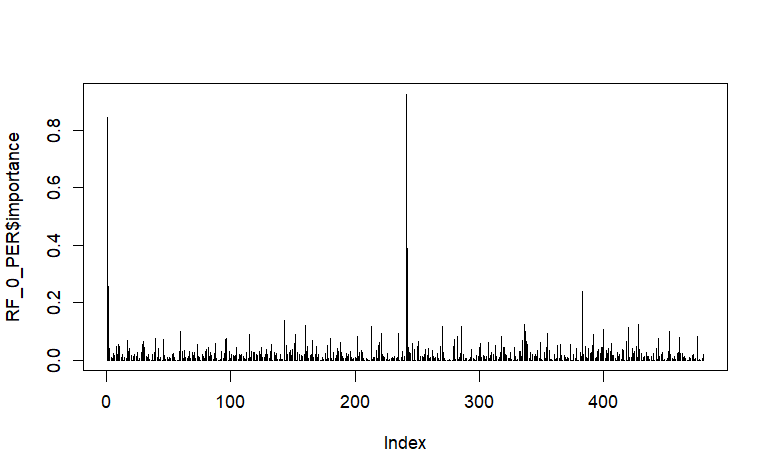
\includegraphics[width=0.45\textwidth]{img/01-5-per.png}}
    \subfigure[\textit{HR\_scaled}]{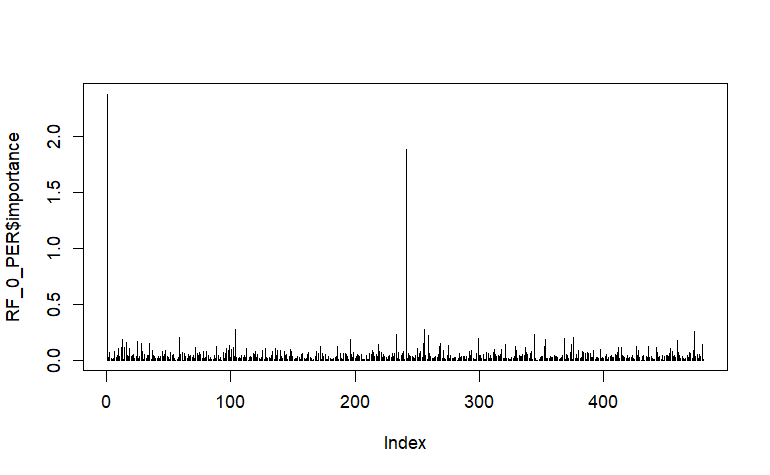
\includegraphics[width=0.45\textwidth]{img/02-5-per.png}}
    \subfigure[\textit{HR\_quantile}]{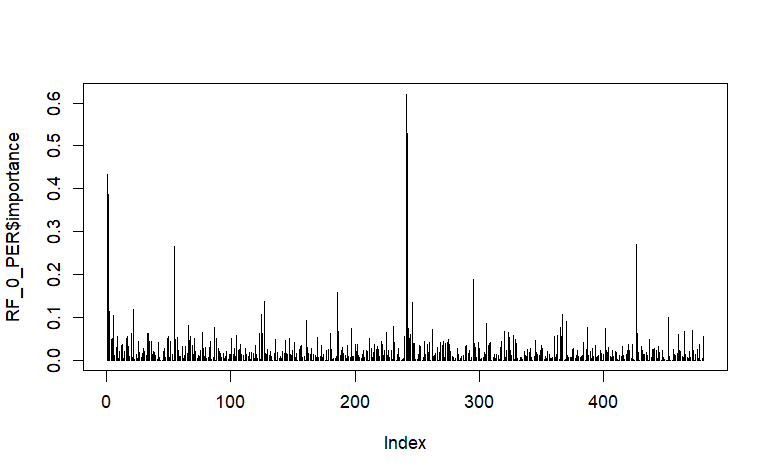
\includegraphics[width=0.5\textwidth]{img/03-5-per.png}}
    \caption{Importancia Peridiograma de \textit{HR}, \textit{HR\_scaled} y \textit{HR\_quantile}}\label{fig:per_imp_fc}
\end{figure}

\begin{figure}[ht]
    \centering
    \subfigure[\textit{SpO2}]{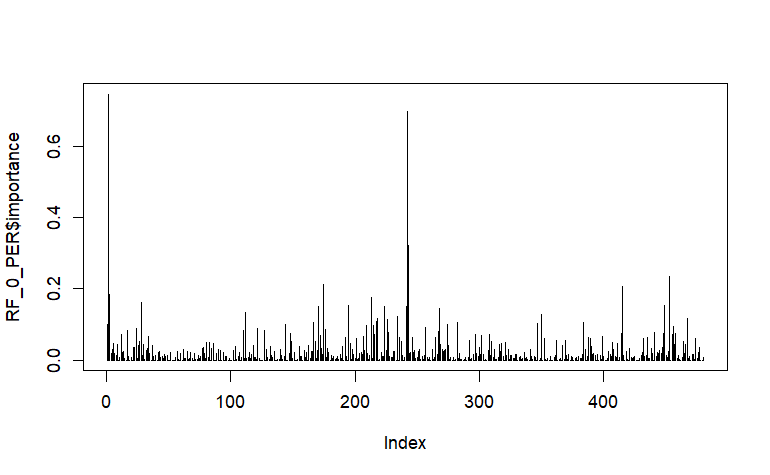
\includegraphics[width=0.5\textwidth]{img/04-5-per.png}}\hfill
    \subfigure[\textit{SpO2\_scaled}]{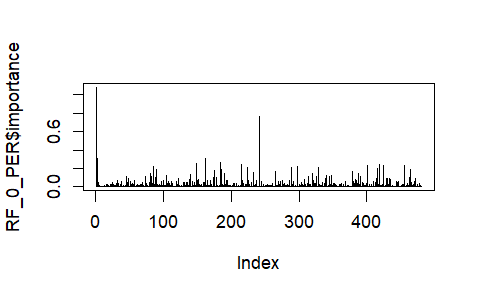
\includegraphics[width=0.5\textwidth]{img/05-5-per.png}}
    \caption{Importancia Peridiograma de \textit{SpO2} y \textit{SpO2\_scaled}}\label{fig:per_imp_spo2}
\end{figure}


\paragraph{Media de los valores de Peridiograma en función de los clusters generados $k = 2$}

\begin{figure}[H]
    \centering
    \subfigure[\textit{HR}]{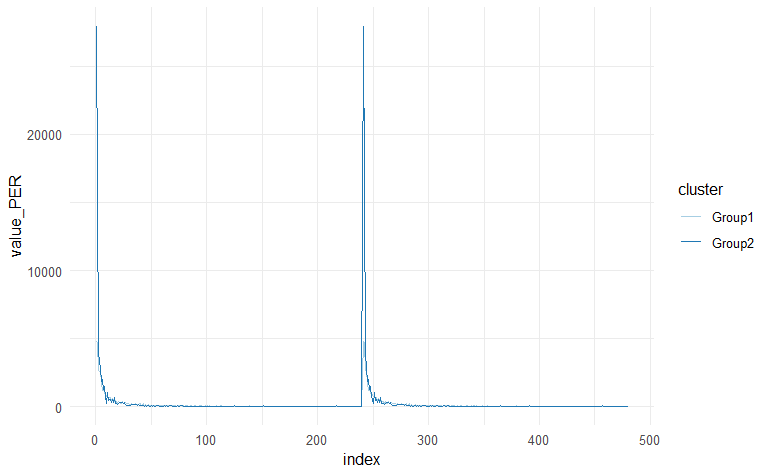
\includegraphics[width=0.45\textwidth]{img/01-6-per.png}}
    \subfigure[\textit{HR\_scaled}]{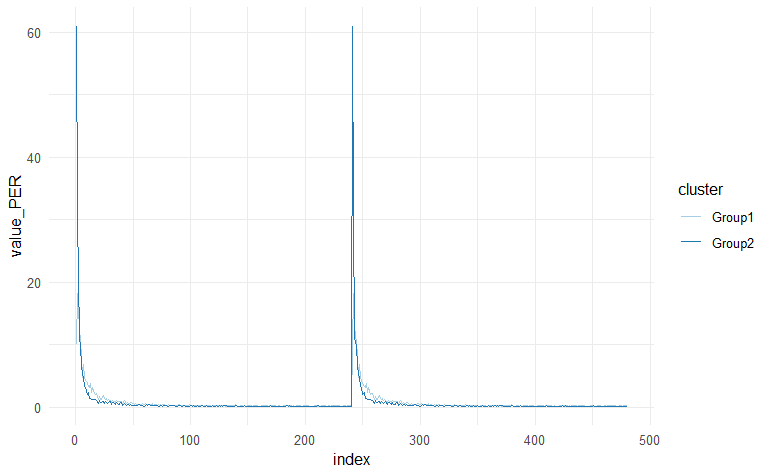
\includegraphics[width=0.45\textwidth]{img/02-6-per.png}}
    \subfigure[\textit{HR\_quantile}]{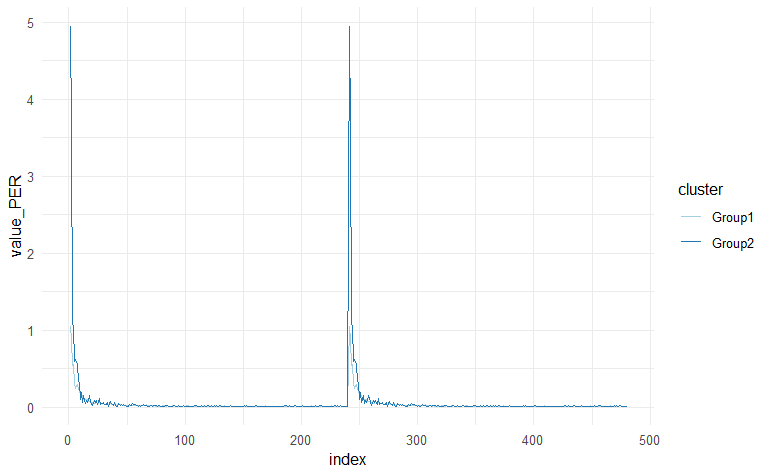
\includegraphics[width=0.5\textwidth]{img/03-6-per.png}}
    \caption{Valores de Peridiograma por cluster k = 2 de \textit{HR}, \textit{HR\_scaled} y \textit{HR\_quantile}}\label{fig:per_cls_fc}
\end{figure}

\begin{figure}[ht]
    \centering
    \subfigure[\textit{SpO2}]{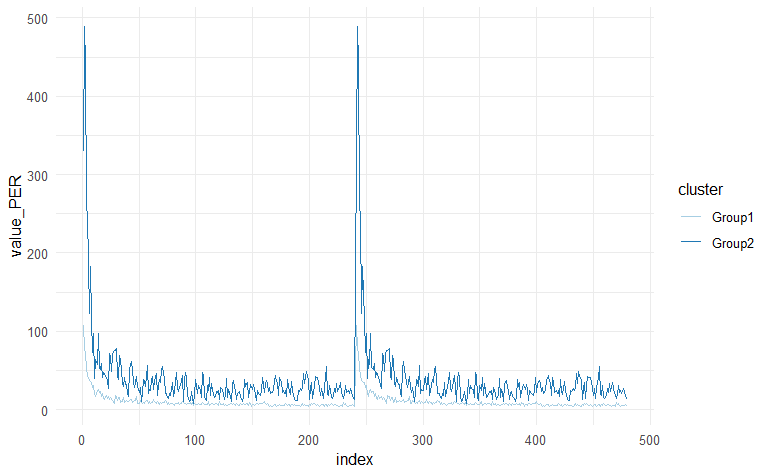
\includegraphics[width=0.5\textwidth]{img/04-6-per.png}}\hfill
    \subfigure[\textit{SpO2\_scaled}]{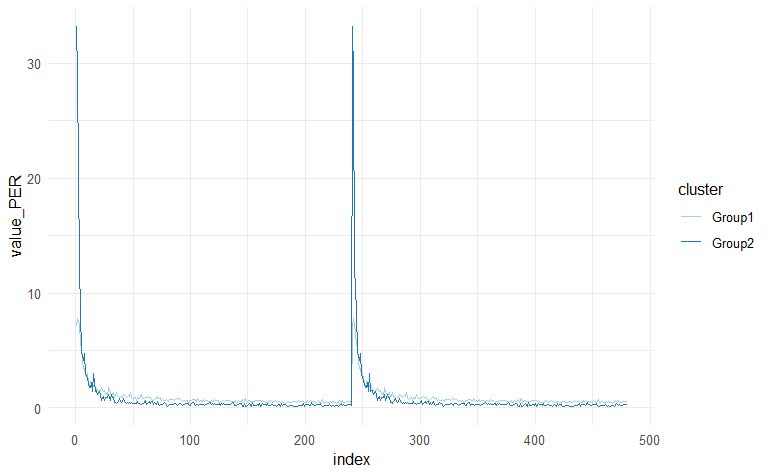
\includegraphics[width=0.5\textwidth]{img/05-6-per.png}}
    \caption{Valores de Peridiograma por cluster k = 2 de \textit{SpO2} y \textit{SpO2\_scaled}}\label{fig:per_cls_spo2}
\end{figure}

